\documentclass[a4paper]{article}
\usepackage{graphicx}
\usepackage{booktabs}
\usepackage{verbatim}
\usepackage{listings}
\lstset{
    basicstyle=\small\ttfamily,
    columns=flexible,
    breakatwhitespace=false,
    breaklines=true
}

\author{Joseph Roberts \\
        \small{jr592}
       }
\title{GF2 Interim Report 2}

\addtolength{\hoffset}{-2cm}
\addtolength{\textwidth}{4cm}
\addtolength{\voffset}{-2cm}
\addtolength{\textheight}{2.5cm}

\begin{document}
\maketitle
\nocite{*}

\section{User guide}
    \subsection{Launching and opening a definition file}
        \begin{enumerate}
            \item Run the executable by either typing \texttt{./bin/runner} from the project directory, or symlinking the executable into one of the folders on your \texttt{PATH} and running it as you would any other program.
            \item To bring up the Open File dialog, either press the hotkey \texttt{ctrl+o}, or navigate the menu bar at the top to \texttt{'File->Open Definition File'}.
        \end{enumerate}

    \subsection{Exploring a definition file}
        The simulator window is broken into three resizeable panes:
        \begin{itemize}
            \item The top left pane is the Network View. Click the arrow to the left of any subnetwork expand its list of components. Double click on any item to bring it up in the Component View.
            \item The top right pane is the ComponentView. A list of the inputs and outputs of the curerntly selected component are shown here.
            \item The bottom pane shows the Plot View. Each monitored signal will generate a trace in this view. You may zoom in and out by scrolling the mouse wheel inside this view, and pan side to side with the scroll bar at the bottom.
        \end{itemize}

    \subsection{Manipulating monitor points}
        It should be noted that if a monitor point for a signal is disabled, all record of the trace is lost. Similarly if a monitor point is added part-way through the simulation, the trace for that point will only begin at that point.
        To add/remove monitor points from the network:

        \begin{enumerate}
            \item Select the component with the signal of interest by double-clicking it in the Network View
            \item Select the output(s) which you wish to monitor/unmonitor in the component view by clicking on them
            \item Click \texttt{'Toggle Monitor Point'} to toggle whether or not the signal is monitored
        \end{enumerate}

    \subsection{Manipulating network inputs (switches)}

        To change the value of Network inputs:
        \begin{enumerate}
            \item Select the Root Network by double clicking on it in the Network View
            \item Select the input(s) that you wish to change by clicking on them in the Component View
            \item Click \texttt{Switch Input State} to toggle the value of each selected input
        \end{enumerate}



\clearpage

\section{Example definition files}
    In this section several example definition files are declared: A 4-bit synchronous counter based on JK flip flops, a full adder, a 4-bit ripple carry adder, and a 4-bit carry lookahead adder.
    The include functionality of our simulator is demonstrated in both of the 4-bit adders (they include the full adder), as well as a further definition called \texttt{4bit-adder-test.def} which includes both the 4-bit adders wired to two synchronous counters as a demonstration.

    To demonstrate how easily these definition files might be generated automatically, an example 16-bit carry lookahead adder is also included. This definition is more than 15000 characters long even with all the spaces and newlines removed. Even larger examples are just as trivial to generate, though would be impractical to include in a report. For instance a 64 bit carry lookahead adder requires nearly half a million characters to define - about 100 pages at the same font size as the 16 bit variant.

    It should be noted that although the following files are in strict lower case, the format is fully case insensitive such that the requirements in the specification about uppercase items are fufilled.
    It should also be noted that the ordering of the keys does not matter.

    \subsection{Full adder}
        \begin{figure}[b]
            \centering
            
\includegraphics[width=0.7\textwidth]{full-adder}
            \caption{Full adder schematic}
        \end{figure}
        \lstinputlisting{full_adder.def}

    \subsection{4 bit synchronous counter}
        \begin{figure}[b]
            \centering
            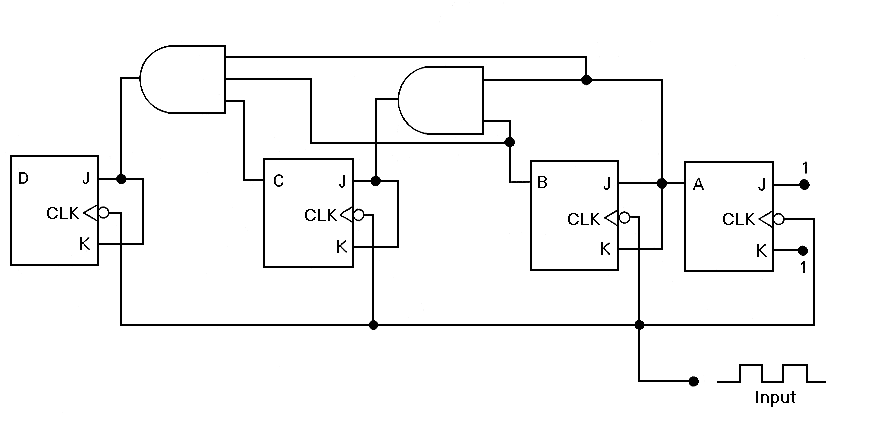
\includegraphics[width=\textwidth]{synchronous-counter}
            \caption{Synchronous counter schematic. Signals marked A, B, C, and D are referenced by the output vector count[4] in the definition}
        \end{figure}
        \lstinputlisting{4bit-synch-counter.def}

    \subsection{4 bit ripple carry adder}
        \begin{figure}[b]
            \centering
            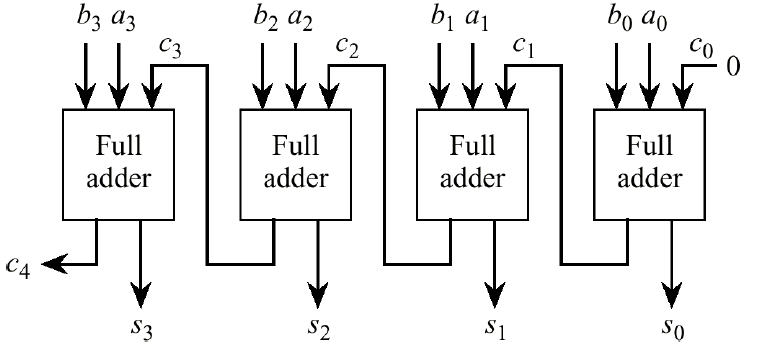
\includegraphics[width=\textwidth]{ripple-carry-adder}
            \caption{Ripple carry adder schematic}
        \end{figure}
        \lstinputlisting{4bit-carry-adder.def}

    \subsection{4 bit carry lookahead adder}
        \begin{figure}[b]
            \centering
            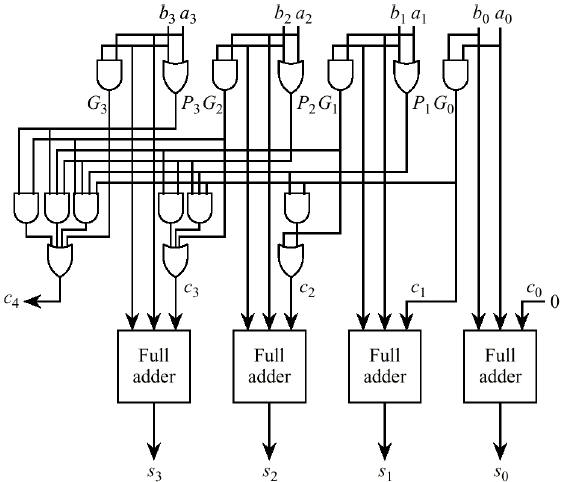
\includegraphics[width=\textwidth]{carry-lookahead-adder}
            \caption{Carry lookahead adder schematic}
        \end{figure}
        \lstinputlisting{4bit-lookahead-adder.def}

    \subsection{4 bit adder test}
        \lstinputlisting{4bit-adder-test.def}

\clearpage

    \subsection{16 bit carry lookahead adder}
        The following definition is stored as a single line with no spaces. Line breaks are inserted here at regular intervals for readability, without regard to whether they intersect a word. Doing so to an actual definition file would prevent it from being parsed.
        \lstinputlisting{16bit-lookahead-adder.def}

\null
\vfill
\bibliographystyle{alpha}
\bibliography{ref}

\end{document}
